\documentclass[oneside]{book}


%pgfpages -  2 pages per sheet
\usepackage{pgfpages}
\pgfpagesuselayout{2 on 1}[a4paper,landscape]
\setlength{\parskip}{1\baselineskip}

% remove header (Deus sabe como)
\usepackage{fullpage}

%\lpobj error  
\usepackage{newtxtext,newtxmath}

% listing code
\usepackage{listings}


%FONT
% \usepackage[utf8]{inputenc}
\usepackage[T1]{fontenc}
\usepackage{fix-cm} 
\usepackage[fontsize=14pt]{fontsize}
\usepackage{geometry}
% \lstset{language={[LaTeX]TeX},basicstyle=\ttfamily}


\newtheorem{theorem}{Theorem}

\usepackage{afterpage}
\newcommand\myemptypage{
    \null
    \thispagestyle{empty}
    \addtocounter{page}{-1}
    \newpage
    }


%Listings
\definecolor{codegreen}{rgb}{0,0.6,0}
\definecolor{codegray}{rgb}{0.5,0.5,0.5}
\definecolor{codepurple}{rgb}{0.58,0,0.82}
\definecolor{backcolour}{rgb}{0.95,0.95,0.92}
\lstdefinestyle{mystyle}{
    backgroundcolor=\color{backcolour},   
    commentstyle=\color{codegreen},
    keywordstyle=\color{magenta},
    %numberstyle=\tiny\color{codegray},
    stringstyle=\color{codepurple},
    basicstyle=\ttfamily\footnotesize,
    breakatwhitespace=false,        
    breaklines=true,                
    captionpos=b,                   
    keepspaces=true,                
    %numbers=left,                   
    %numbersep=5pt,                  
    showspaces=false,               
    showstringspaces=false,
    showtabs=false,                 
    tabsize=2
}

\lstset{style=mystyle}
\usepackage[tikz]{bclogo}

\usepackage{pdfpages}

\usepackage{tikz}
\usetikzlibrary{shapes.geometric, arrows}
\usetikzlibrary{calc}
\usetikzlibrary{positioning}
\tikzstyle{lpnode} = [align=center]
\tikzstyle{arrow} = [thick,->,>=stealth,text width=3.5cm, align=center]
\usetikzlibrary{arrows,positioning} 
   \usetikzlibrary{arrows.meta}
\tikzset{
    %Define standard arrow tip
    >=stealth',
    %Define style for boxes
    punkt/.style={
           rectangle,
           rounded corners,
           draw=black, very thick,
           text width=6.5em,
           minimum height=2em,
           text centered},
    % Define arrow style
    pil/.style={
           ->,
           thick,
           shorten <=2pt,
           shorten >=2pt,}
}

\newcommand{\tm}[2]{%
     \tikz[overlay,remember picture,baseline] \node [anchor=base] (#1) {$#2$};%
}


\usepackage{algorithm} 
\usepackage{algorithmicx} 
\usepackage{algpseudocode}
% \usepackage{xcolor}
% \usepackage[linesnumbered,ruled,vlined]{algorithm2e}

% \newcommand\mycommfont[1]{\footnotesize\ttfamily\textcolor{blue}{#1}}
% \SetCommentSty{mycommfont}

% \SetKwInput{KwInput}{Input}                % Set the Input
% \SetKwInput{KwOutput}{Output}              % set the Output


% Sanming
\newcommand{\blue}{\textcolor{blue}}
\newcommand{\green}{\textcolor{green}}
\newcommand{\red}{\textcolor{red}}
\newcommand{\purple}{\textcolor{purple}}
\newcommand{\be}{\begin{equation}}
\newcommand{\ee}{\end{equation}}
\newcommand{\ben}{\begin{equation*}}
\newcommand{\een}{\end{equation*}}
% \newcommand{\bea}{\begin{eqnarray}}
% \newcommand{\eea}{\end{eqnarray}}
\newcommand{\bean}{\begin{eqnarray*}}
\newcommand{\eean}{\end{eqnarray*}}
\newcommand{\amat}[2]{\left[\begin{matrix}#1\end{matrix}\,\,\right|\left.\begin{matrix}#2\end{matrix}\right]}
\newcommand{\bmat}[1]{\begin{bmatrix}#1\end{bmatrix}}
\newcommand{\dmat}[1]{\begin{vmatrix}#1\end{vmatrix}}
\newcommand{\tablefont}{\footnotesize}


\usepackage{csvsimple}
\usepackage{bibentry}
\usepackage[colorlinks=true,linkcolor=blue,urlcolor=blue,citecolor=blue,plainpages=false]{hyperref}
\usepackage{ lpform }
\usepackage{subfiles}

%MAST 20018

%New commands for matrices


\usepackage{subfigure}
\usepackage{caption}
\usepackage{multicol}
\setlength{\parindent}{0pt}

\usepackage{pgfplots}
\pgfplotsset{compat=1.16}
\usepackage{booktabs}



\begin{document}
\bibliographystyle{apalike}



%%%%%%%%%%%%%%%  COVER %%%%%%%%%%%%%%%
\begin{titlepage}

\begin{center}
% \textsc{\LARGE The University  of Melbourne}\\[0.2cm]
% \textsc{\Large School of Mathematics and Statistics}\\[0.5cm] 

\vfill

\rule{\linewidth}{0.5mm} \\[0.4cm]
\textsc{\Large OPTIMA Graduate Research Workshop \\[0.4cm] On  Benders decomposition }
\rule{\linewidth}{0.5mm} \\[1.5cm]

\end{center}

{\large 
\noindent Andreas Ernst\\[.3cm]
\noindent Alysson M. Costa\\
}

\vfill 

\includegraphics[width=8cm]{fig/optima.png}

\vspace{2cm}
% \date{May 29, 2023}  

\end{titlepage}

%%%%%%%%%%%%%%%  END COVER %%%%%%%%%%%%%%%

\section*{}

\vfill

Mixed-Integer Programming (MIP) is a highly effective method for solving optimisation problems. The remarkable progress made by MIP solvers such as CPLEX and GUROBI in the last three decades has resulted in the widespread use of the technique as the approach of choice for tackling many industrial applications.

The complexity of some industrial applications exceeds the capabilities of these solvers. In order to advance the use of MIP, decomposition techniques are a popular approach. These methods divide the problem into smaller sub-problems that fall into the solvers reach. Benders decomposition is one of the most successful techniques in this regard.

In this workshop, we provide a gentle introduction to the core concepts of Benders decomposition. This includes a hands-on tutorial on implementing an algorithm for a toy problem. In the second part of the workshop, we will discuss recent advances in the field and exemplify how the technique can be applied to solve large-scale industrial problems.

Participants are requested to bring their laptops and register for an account at Google Colaboratory (https://colab.research.google.com/) in order to participate in the hands-on tutorial.

\vfill

\newpage





\subsection*{Mixed-Integer Programming}

\vfill

\begin{align*}
\textrm{Maximise } \quad &  c^tx + d^ty \\
\textrm{s.t.} \quad & Ax + By \geq b, \\
& Dy \geq e, \\
& x {\geq 0},  y {\geq 0} \textrm{ and integer}.\\
\end{align*}
%
\vfill
\begin{bclogo}[logo=\bccrayon]{\small Example } \small
\vspace{-0.5cm}
\begin{align*}
\textrm{Maximise} \quad   x_1 &- x_2 + y_1 + y_2 \\
\textrm{s.t.} \quad  -x_1 & - x_2 - y_2 \geq -2, \\
 x_1  &+ x_2 - y_1 \geq 1, \\
y_1, & y_2 \leq 2, \\
 x_1, & x_2 \geq 0, \\
 y_1, & y_2 \in \{0,1\}.
\end{align*}
\end{bclogo}
\vfill
\begin{bclogo}[logo=\bcinfo, barre=none ]{\small Implementation}
\vspace{0.2cm}
\lstinputlisting[language=python,basicstyle=\tiny]{code/toyExampleInteger.py}
\end{bclogo}
\vfill


\newpage

\subsection*{}

\begin{bclogo}[logo=\bcvaletcoeur]{\small \vspace{.2cm} Give me a list of applications of Mixed-Integer Programming}
\vspace{.2cm}

\footnotesize

\begin{enumerate}
\item \textbf{Production planning}: Mixed-Integer Programming can be used to optimize production planning, such as determining the optimal mix of products to manufacture or the best schedule for production runs.
\item \textbf{Supply chain management}: Mixed-Integer Programming can be used to optimize supply chain decisions, such as transportation and inventory management.
\item \textbf{Facility location and network design}: Mixed-Integer Programming can be used to determine the optimal location of facilities and the design of supply chain networks.
\item \textbf{Resource allocation}: Mixed-Integer Programming can be used to optimize resource allocation decisions, such as the allocation of labor and equipment.
\item \textbf{Financial planning and portfolio optimization}: Mixed-Integer Programming can be used to optimize financial planning and portfolio optimization decisions, such as asset allocation and investment selection.
\item \textbf{Energy and environmental systems}: Mixed-Integer Programming can be used to optimize energy systems, such as the design and operation of power grids, and to optimize environmental systems, such as waste management and pollution reduction.
\item \textbf{Telecommunications and network optimization}: Mixed-Integer Programming can be used to optimize network design and routing decisions, such as the placement of cell towers and the routing of network traffic.
\item \textbf{Healthcare management}: Mixed-Integer Programming can be used to optimize healthcare decisions, such as the allocation of hospital resources and the design of clinical trials.
\item \textbf{Transportation and logistics}: Mixed-Integer Programming can be used to optimize transportation and logistics decisions, such as route optimization and vehicle scheduling.
\item \textbf{Scheduling and timetabling}: Mixed-Integer Programming can be used to optimize scheduling and timetabling decisions, such as employee scheduling and course timetabling.
\end{enumerate}

\vspace{.2cm}
\end{bclogo}
\vspace{1cm}




\newpage


\begin{center}
\centering
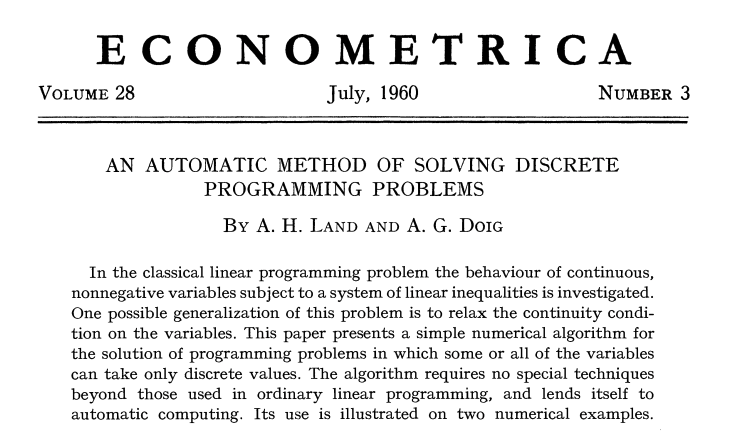
\includegraphics[width=12cm]{fig/econometrica.png}
\end{center}



{\tiny

\begin{verbatim}
                    Username
                    Academic license - for non-commercial use only - expires 2023-11-04
                    Gurobi Optimizer version 9.5.0 build v9.5.0rc5 (mac64[x86])
                    Thread count: 4 physical cores, 8 logical processors, using up to 8 threads
                    Optimize a model with 2 rows, 4 columns and 6 nonzeros
                    Model fingerprint: 0x252cfa2e
                    Variable types: 2 continuous, 2 integer (2 binary)
                    Coefficient statistics:
                      Matrix range     [1e+00, 1e+00]
                      Objective range  [1e+00, 1e+00]
                      Bounds range     [1e+00, 1e+00]
                      RHS range        [1e+00, 2e+00]
                    Presolve removed 2 rows and 4 columns
                    Presolve time: 0.00s
                    Presolve: All rows and columns removed
                    
                    Explored 0 nodes (0 simplex iterations) in 0.00 seconds (0.00 work units)
                    Thread count was 1 (of 8 available processors)
                    
                    Solution count 1: 3 
                    
                    Optimal solution found (tolerance 1.00e-04)
                    Best objective 3.000000000000e+00, best bound 3.000000000000e+00, gap 0.0000%
                    x[1] =  2.0
                    x[2] =  0.0
                    y[1] =  1.0
                    y[2] =  0.0
                    Optimal solution value: 3.0
                    [Finished in 0.5s]
\end{verbatim}
}


\newpage

\subsection*{Benders decomposition}



For many years, Benders decomposition \cite{benders62partitioning}  was a brilliant theoretical result with little applicability in practice. 


\begin{center}

\includegraphics[width=14cm]{fig/fig1}
\end{center}


\newpage

\subsection*{Industrial applications}


It took 12 years for Benders decomposition to be first used on a practical application  \cite{geoffrion74multicommodity}. 


\begin{center}
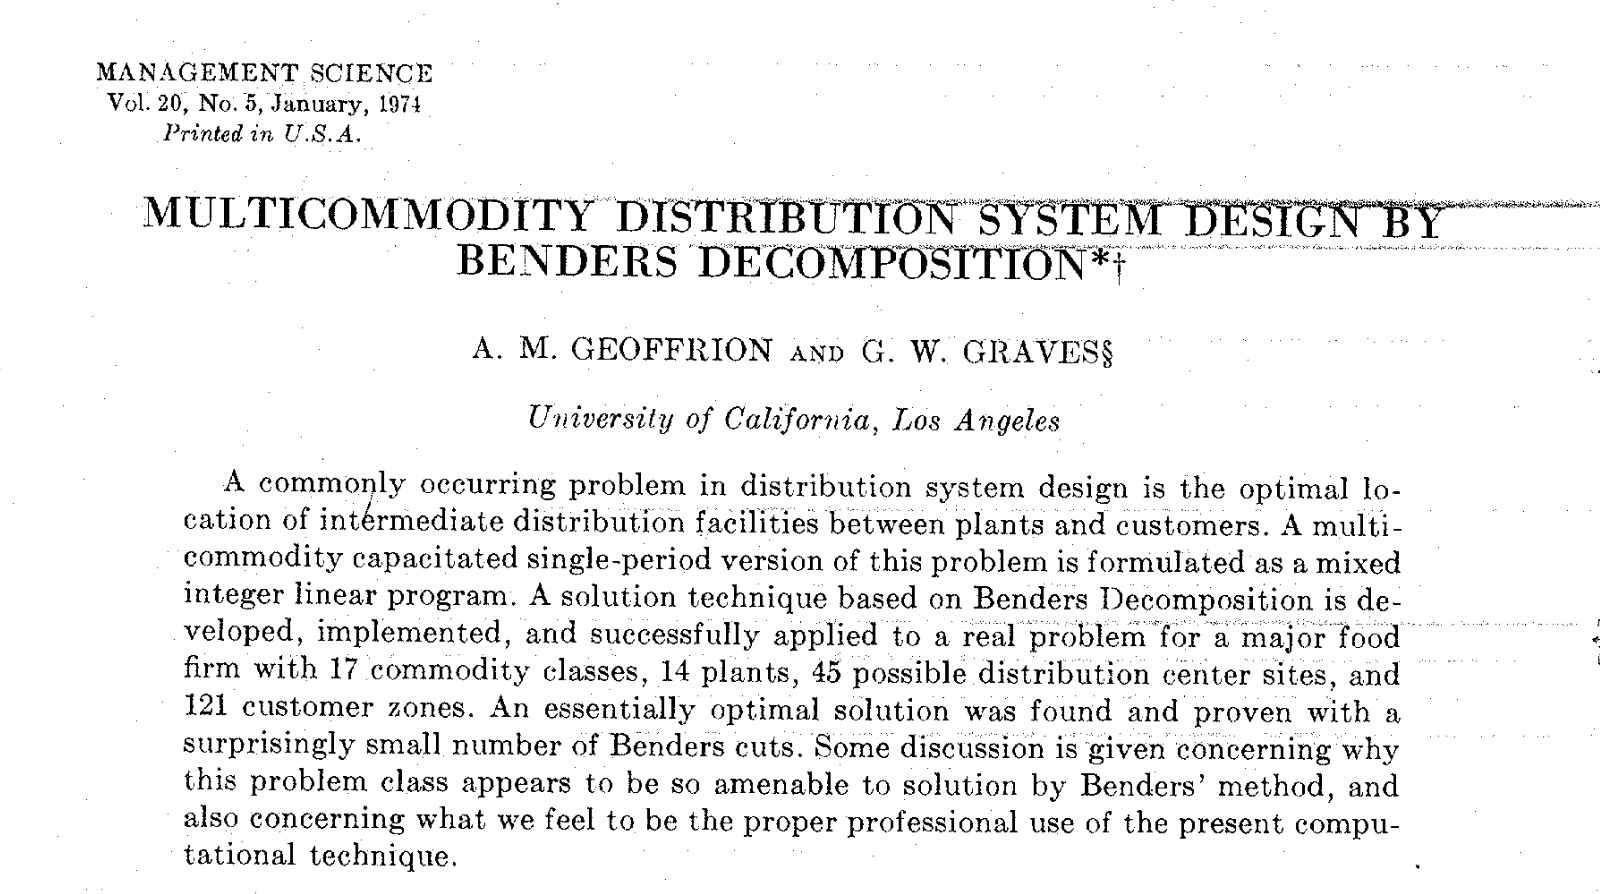
\includegraphics[width=14cm]{fig//fig2}
\end{center}


\begin{center}
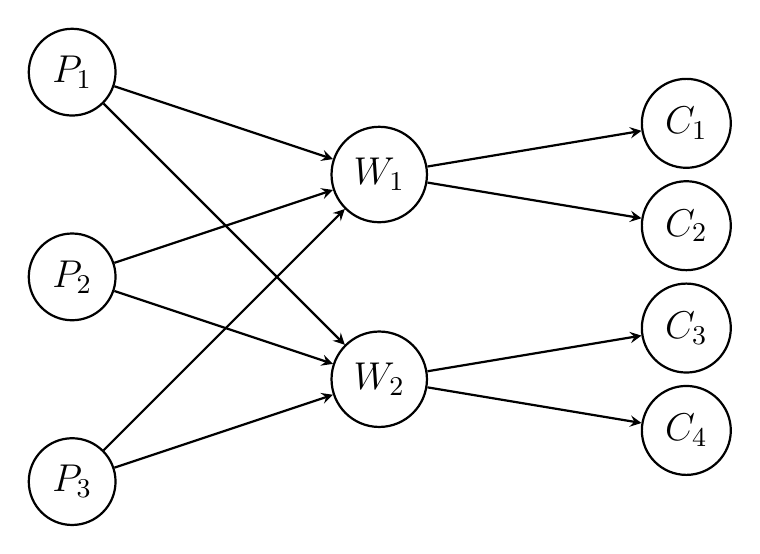
\begin{tikzpicture}[scale=1.3,thick,>=stealth]

% Nodes
\node[draw, circle] (p1) at (0,0) {$P_1$};
\node[draw, circle] (p2) at (0,-2) {$P_2$};
\node[draw, circle] (p3) at (0,-4) {$P_3$};
\node[draw, circle] (w1) at (3,-1) {$W_1$};
\node[draw, circle] (w2) at (3,-3) {$W_2$};
\node[draw, circle] (c1) at (6,-0.5) {$C_1$};
\node[draw, circle] (c2) at (6,-1.5) {$C_2$};
\node[draw, circle] (c3) at (6,-2.5) {$C_3$};
\node[draw, circle] (c4) at (6,-3.5) {$C_4$};

% Edges
\draw[->] (p1) -- node[midway, above] {$$} (w1);
\draw[->] (p1) -- node[midway, below] {$$} (w2);
\draw[->] (p2) -- node[midway, above] {$$} (w1);
\draw[->] (p2) -- node[midway, below] {$$} (w2);
\draw[->] (p3) -- node[midway, above] {$$} (w1);
\draw[->] (p3) -- node[midway, below] {$$} (w2);
\draw[->] (w1) -- node[midway, above] {$$} (c1);
\draw[->] (w1) -- node[midway, above] {$$} (c2);
\draw[->] (w2) -- node[midway, above] {$$} (c3);
\draw[->] (w2) -- node[midway, above] {$$} (c4);

\end{tikzpicture}
\end{center}

\newpage


% Benders decomposition is often the decomposition technique of choice in Mixed-Integer Programming \cite{costa05survey,rahmaniani17benders}.

\subsection*{The Benders reformulation}

Consider again a generic MIP model:
\begin{align*}
    \textrm{Maximise } \quad &  c^tx + d^ty  \\
    \textrm{s.t.} \quad & Ax + By \geq b,  \\
                    & Dy \geq e,  \\
                    & x \geq 0, y \geq 0 \textrm{ and integer.}  
\end{align*}






\vfill


 This problem can be rewritten as:
\begin{eqnarray*}
\label{bd2}  \textrm{Maximise}_{\, y \in Y \,} \{\,
d^ty + \textrm{Maximise}_{\, x\geq 0 \,} \{ c^tx  : Ax \leq b -
By\}\, \},
\end{eqnarray*}

with $Y = \{ y \, |\, Dy \geq e, \,\, y \geq 0
\textrm{ and integer} \}$.
\vspace{1cm}


The inner problem is a linear programming model and is known as the Benders decomposition subproblem.

\vfill

Now consider a tentative solution $\overline{y}$. Associating dual variables $u$ to constraints $Ax \geq
b-B\overline{y}$, we can write the dual version of  subproblem as
\begin{eqnarray*}
\label{bd3}  \textrm{Minimise}_{\, u\geq 0 \,} \{ u^t(b-B\overline{y}) :
u^tA \geq c\}.
\end{eqnarray*}

\vfill


\newpage

\subsection*{}

Let  $\mathbb{F} = \{ u \, |\, u \geq 0 \,\, ; \, \, u^tA \geq c \}$.  We assume that $\mathbb{F}$ is not empty for it would correspond to a primal problem either infeasible or
unbounded. 

$\mathbb{F}$ is therefore composed of extreme points $u^p$ (for
$p=1 \dots P$) and extreme rays $r^q$ (for $q=1 \dots Q$).\\


\begin{bclogo}[logo=\bccrayon]{\small Example }
\small \vspace{-.5cm}
\begin{align*}
\textrm{Minimise} \quad &  (2-\overline{y}_2)u_1 + (-1 - \overline{y}_1)u_2 \\
& u_1 -  u_2  \geq 1, \\
& u_1 -u_2 \geq -1, \\
& u_1, u_2 \geq 0.
\end{align*}

\end{bclogo}




\begin{center}
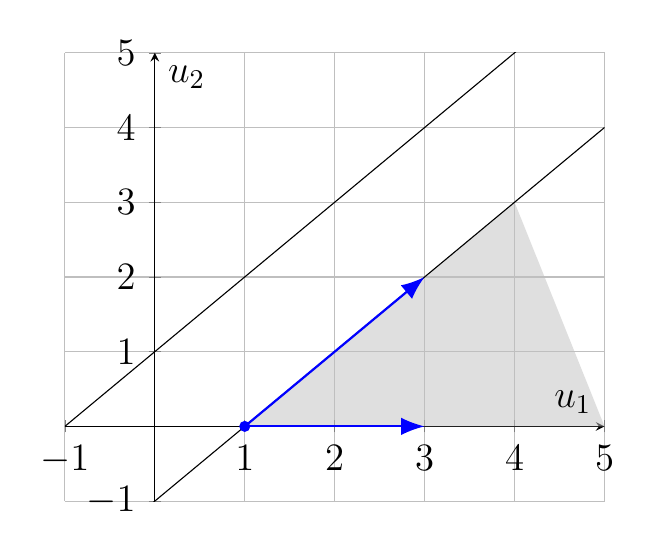
\begin{tikzpicture}[scale=1]
\begin{axis}[
  axis lines=center,
  xlabel=$u_1$,
  ylabel=$u_2$,
  xmin=-1, xmax=5,
  ymin=-1, ymax=5,
  xtick={-1,0,1,...,5},
  ytick={-1,0,1,...,5},
  grid=major,
  legend pos=outer north east
]

% Feasible region
\fill[gray!50, opacity=0.5] (1,0) -- (5,0) -- (4,3)  -- cycle;
\addplot[domain=-1:5] {(x-1) };
\addplot[domain=-1:5] {(x+1) };

  % rays
\draw[-{Latex[length=3mm]}, blue, thick] (1,0) -- (3, 2) ;
\draw[-{Latex[length=3mm]}, blue, thick] (1,0) -- (3, 0) ;

% extreme points
\fill[blue] (1, 0) circle (2pt) node[above left] {$$};


\end{axis}
\end{tikzpicture}
\end{center}


\newpage
\subsection*{}


Using duality theory, the primal and dual formulations can be interchanged.
\begin{eqnarray*}
\label{bd4}  \textrm{Maximise}_{\, \overline{y} \in Y \,} \{\,
d^t\overline{y} + \textrm{Minimise}_{\, u\geq 0 \,} \{ u^t(b-B\overline{y})
: u^tA \geq c\}\, \}.
\end{eqnarray*}
The feasible space of the dual subproblem does not depend on the choice of~$\overline{y}$.

\vfill

 The objective function of the subproblem depends on the choice ~$\overline{y}$ and can be either bounded or unbounded. 


\begin{center}
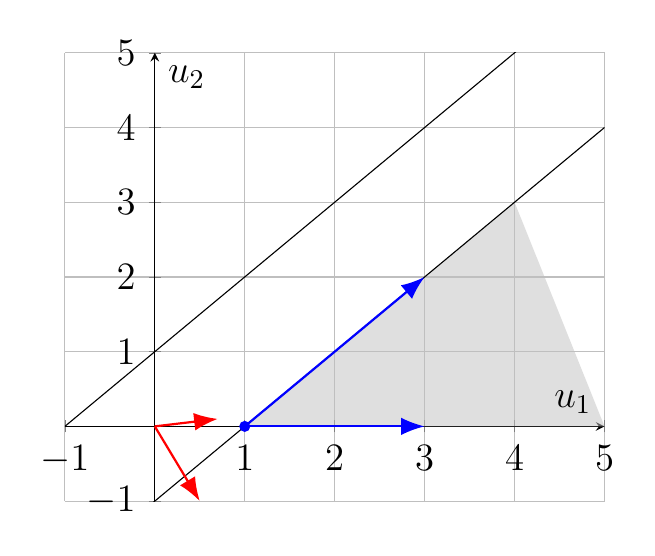
\begin{tikzpicture}[scale=1]
\begin{axis}[
  axis lines=center,
  xlabel=$u_1$,
  ylabel=$u_2$,
  xmin=-1, xmax=5,
  ymin=-1, ymax=5,
  xtick={-1,0,1,...,5},
  ytick={-1,0,1,...,5},
  grid=major,
  legend pos=outer north east
]

% Feasible region
\fill[gray!50, opacity=0.5] (1,0) -- (5,0) -- (4,3)  -- cycle;
\addplot[domain=-1:5] {(x-1) };
\addplot[domain=-1:5] {(x+1) };

  % rays
\draw[-{Latex[length=3mm]}, blue, thick] (1,0) -- (3, 2) ;
\draw[-{Latex[length=3mm]}, blue, thick] (1,0) -- (3, 0) ;

% extreme points
\fill[blue] (1, 0) circle (2pt) node[above left] {$$};


% Gradients
\draw[-{Latex[length=3mm]}, red, thick] (0,0) -- (.5, -1) ;
\draw[-{Latex[length=3mm]}, red, thick] (0,0) -- (.7, 0.1) ;




\end{axis}
\end{tikzpicture}
\end{center}

\vfill


In the first case, we obtain an extreme point $u^p$. In the latter situation, there is a direction $r^q$ for which $r^q(b-B\overline{y}) > 0$.  This direction is either extreme or a convex combination of extreme directions \cite{costa09benders}. \footnote{To simplify the notation in the following, assume that $r^q$ and $u^p$ are row vectors.}
\vfill


\newpage
\subsection*{}

A tentative solution $\overline{y}$ that provides an unbounded  solution to the dual subproblem  implies an infeasible  subproblem and must be avoided.  This is done by  adding  constraints:
\begin{equation}
\label{feascuts}
r^q(b-B\overline{y}) \leq 0, \qquad q=1 \dots Q.
\end{equation}



\begin{bclogo}[logo=\bccrayon]{\small Example:  $y = (1,1)$ }
\small \vspace{-.5cm}
\begin{align*}
\textrm{Minimise} \quad &  u_1 - 2u_2 \\
\textrm{s.t.} \quad & u_1 -  u_2  \geq 1, \\
& u_1 -u_2 \geq -1, \\
& u_1, u_2 \geq 0.
\end{align*}
\end{bclogo}

Adding  constraints \eqref{feascuts} to the  formulation.
\vspace{-0.5cm}

\begin{align*}
\textrm{Maximise}_{\, \overline{y} \in Y \,}  & \, d^ty + \{ \textrm{Minimise}_{\, u\geq 0 \,} \{ u(b-B\overline{y})
: uA \geq c\}\, \\
\textrm{s.t.} \quad & r^q(b-By) \leq 0.
\end{align*}

Now the solution must be one of the extreme points $u_p, \, p=1,\hdots,P. $
\vspace{-0.5cm}

\begin{align*}
\textrm{Maximise}_{\, \overline{y} \in Y \,}  & \,  d^ty + \{ \textrm{Minimise}\{u^p(b-By): p=1,\hdots,P \} \\
\textrm{s.t.} \quad & r^q(b-By) \leq 0, \quad  q=1,\hdots,Q.
\end{align*}

Which can be linearised with the use of a continuous variable $z$ as:
\vspace{-0.5cm}

\begin{align*}
\textrm{Maximise}_{\, \overline{y} \in Y \,}  & \,  d^ty + \{ \textrm{Minimise}\{u^p(b-By): p=1,\hdots,P \} \\
\textrm{s.t.} \quad & r^q(b-By) \leq 0, \quad  q=1,\hdots,Q,\\
& z \leq u^p(b-By), \quad  p=1,\hdots,P.
\end{align*}



This is the \textbf{Benders reformulation}. 

%and its drawback is that the number of extreme
%points and extreme rays is usually extremely large. To overcome
%this limitation, Benders proposed to delay the generation of
%constraints (\ref{bd8}) and (\ref{bd9}). Initially, only
%constraints (\ref{bd10}) are considered, yielding the first master
%problem:

\newpage

\subsection*{Benders decomposition algorithm}

The idea of the \textbf{Benders decomposition algorithm} is to ignore most of the initial constraints of the Benders reformulation and generate them as needed. 

We start with a relaxed version of the reformulation called the \emph{relaxed master problem.}
\begin{align*}
\textrm{Maximise}_{\, \overline{y} \in Y \,}  & \,  d^ty + z \\
\textrm{s.t.} \quad & z \geq -M.
\end{align*}
\vspace{-.2cm}
This gives us tentative values for the integer variables, $\overline{y}$, that are sent to the subproblem:
\begin{align*}
\textrm{Minimise}_{\, u \geq 0 \,}  & \,  u^t(b-B\overline{y}) \\
\textrm{s.t.} \quad & uA \geq c.
\end{align*}
which returns us an extreme ray $r^q$ or an extreme point $u^p$ that can be used to generate a feasibility or optimality cut for the master problem (and the method iterates). 

\vfill

\subsection*{Convergence}

Every time the Master problem is run, we have a dual bound for the problem (i.e., we have solved a relaxation of the problem). Every time the subproblem finds an extreme point, we have found a primal bound for the problem (i.e.,we have found a feasible solution). 

The method converges when the last dual bound found is equal (up to a tolerance) to the best primal bound found during the process. 

\vfill


\subsection*{Improving convergence}

There are many ways to fasten the convergence of a Benders decomposition algorithm \cite{mcdaniel77modified,magnanti81accelerating,papadakos08practical,costa12accelerating,crainic21partial} 

See \cite{costa05survey,rahmaniani17benders} for surveys.


\newpage

\begin{bclogo}[logo=\bccrayon]{\small Example }
\vspace{.2cm} \small


Solve the optimisation problem below using Benders decomposition
\begin{align*}
\textrm{Maximise} \quad &  x_1 - x_2 + y_1 + y_2 \\
\textrm{s.t.} \quad & -x_1 - x_2 - y_2 \geq -2, \\
& x_1 +  x_2 - y_1 \geq 1, \\
& x_1, x_2 \geq 0, \\
& y_1, y_2 \in \{0,1\}.
\end{align*}
\end{bclogo}
\vspace{0.1cm}

\newpage

\subsection*{}

\begin{bclogo}[logo=\bcinfo]{\small Master Problem template:}
\vspace{.2cm} \tiny
\lstinputlisting[language=python]{code/BendersMasterTemplate.py}
\end{bclogo}



\begin{bclogo}[logo=\bcinfo]{\small Subproblem template:}
\vspace{.2cm} \tiny

\lstinputlisting[language=python]{code/BendersSubproblemTemplate.py}

\end{bclogo}

\newpage

\subsection*{}


\begin{bclogo}[logo=\bcinfo]{\small External loop template:}
\vspace{.2cm} \tiny

\lstinputlisting[language=python]{code/BendersTemplate.py}


\vspace{.2cm}
\end{bclogo}


\newpage
\begin{bclogo}[logo=\bcinfo]{\small An implementation using lazy constraints:}
\vspace{.2cm} \tiny

\lstinputlisting[language=python]{code/BendersLazy.py}


\vspace{.2cm}
\end{bclogo}

\newpage

\bibliography{OptimaGRWorkshop}     
\end{document}
